Les figures ci-après représentent des essais de lissage avec le filtre de Savitzky-Golay sur quelques pixels appartenant aux parcelles suivies. Pour chaque pixel, nous faisons varier sur les colonnes le degré du polynôme d'ajustement et sur les lignes la largeur de la fenêtre de lissage, selon les valeurs proposées dans la littérature notamment par \citet{Chen2004}. 

\vspace{5mm}

\begin{figure}[htbp]
 \begin{center}
  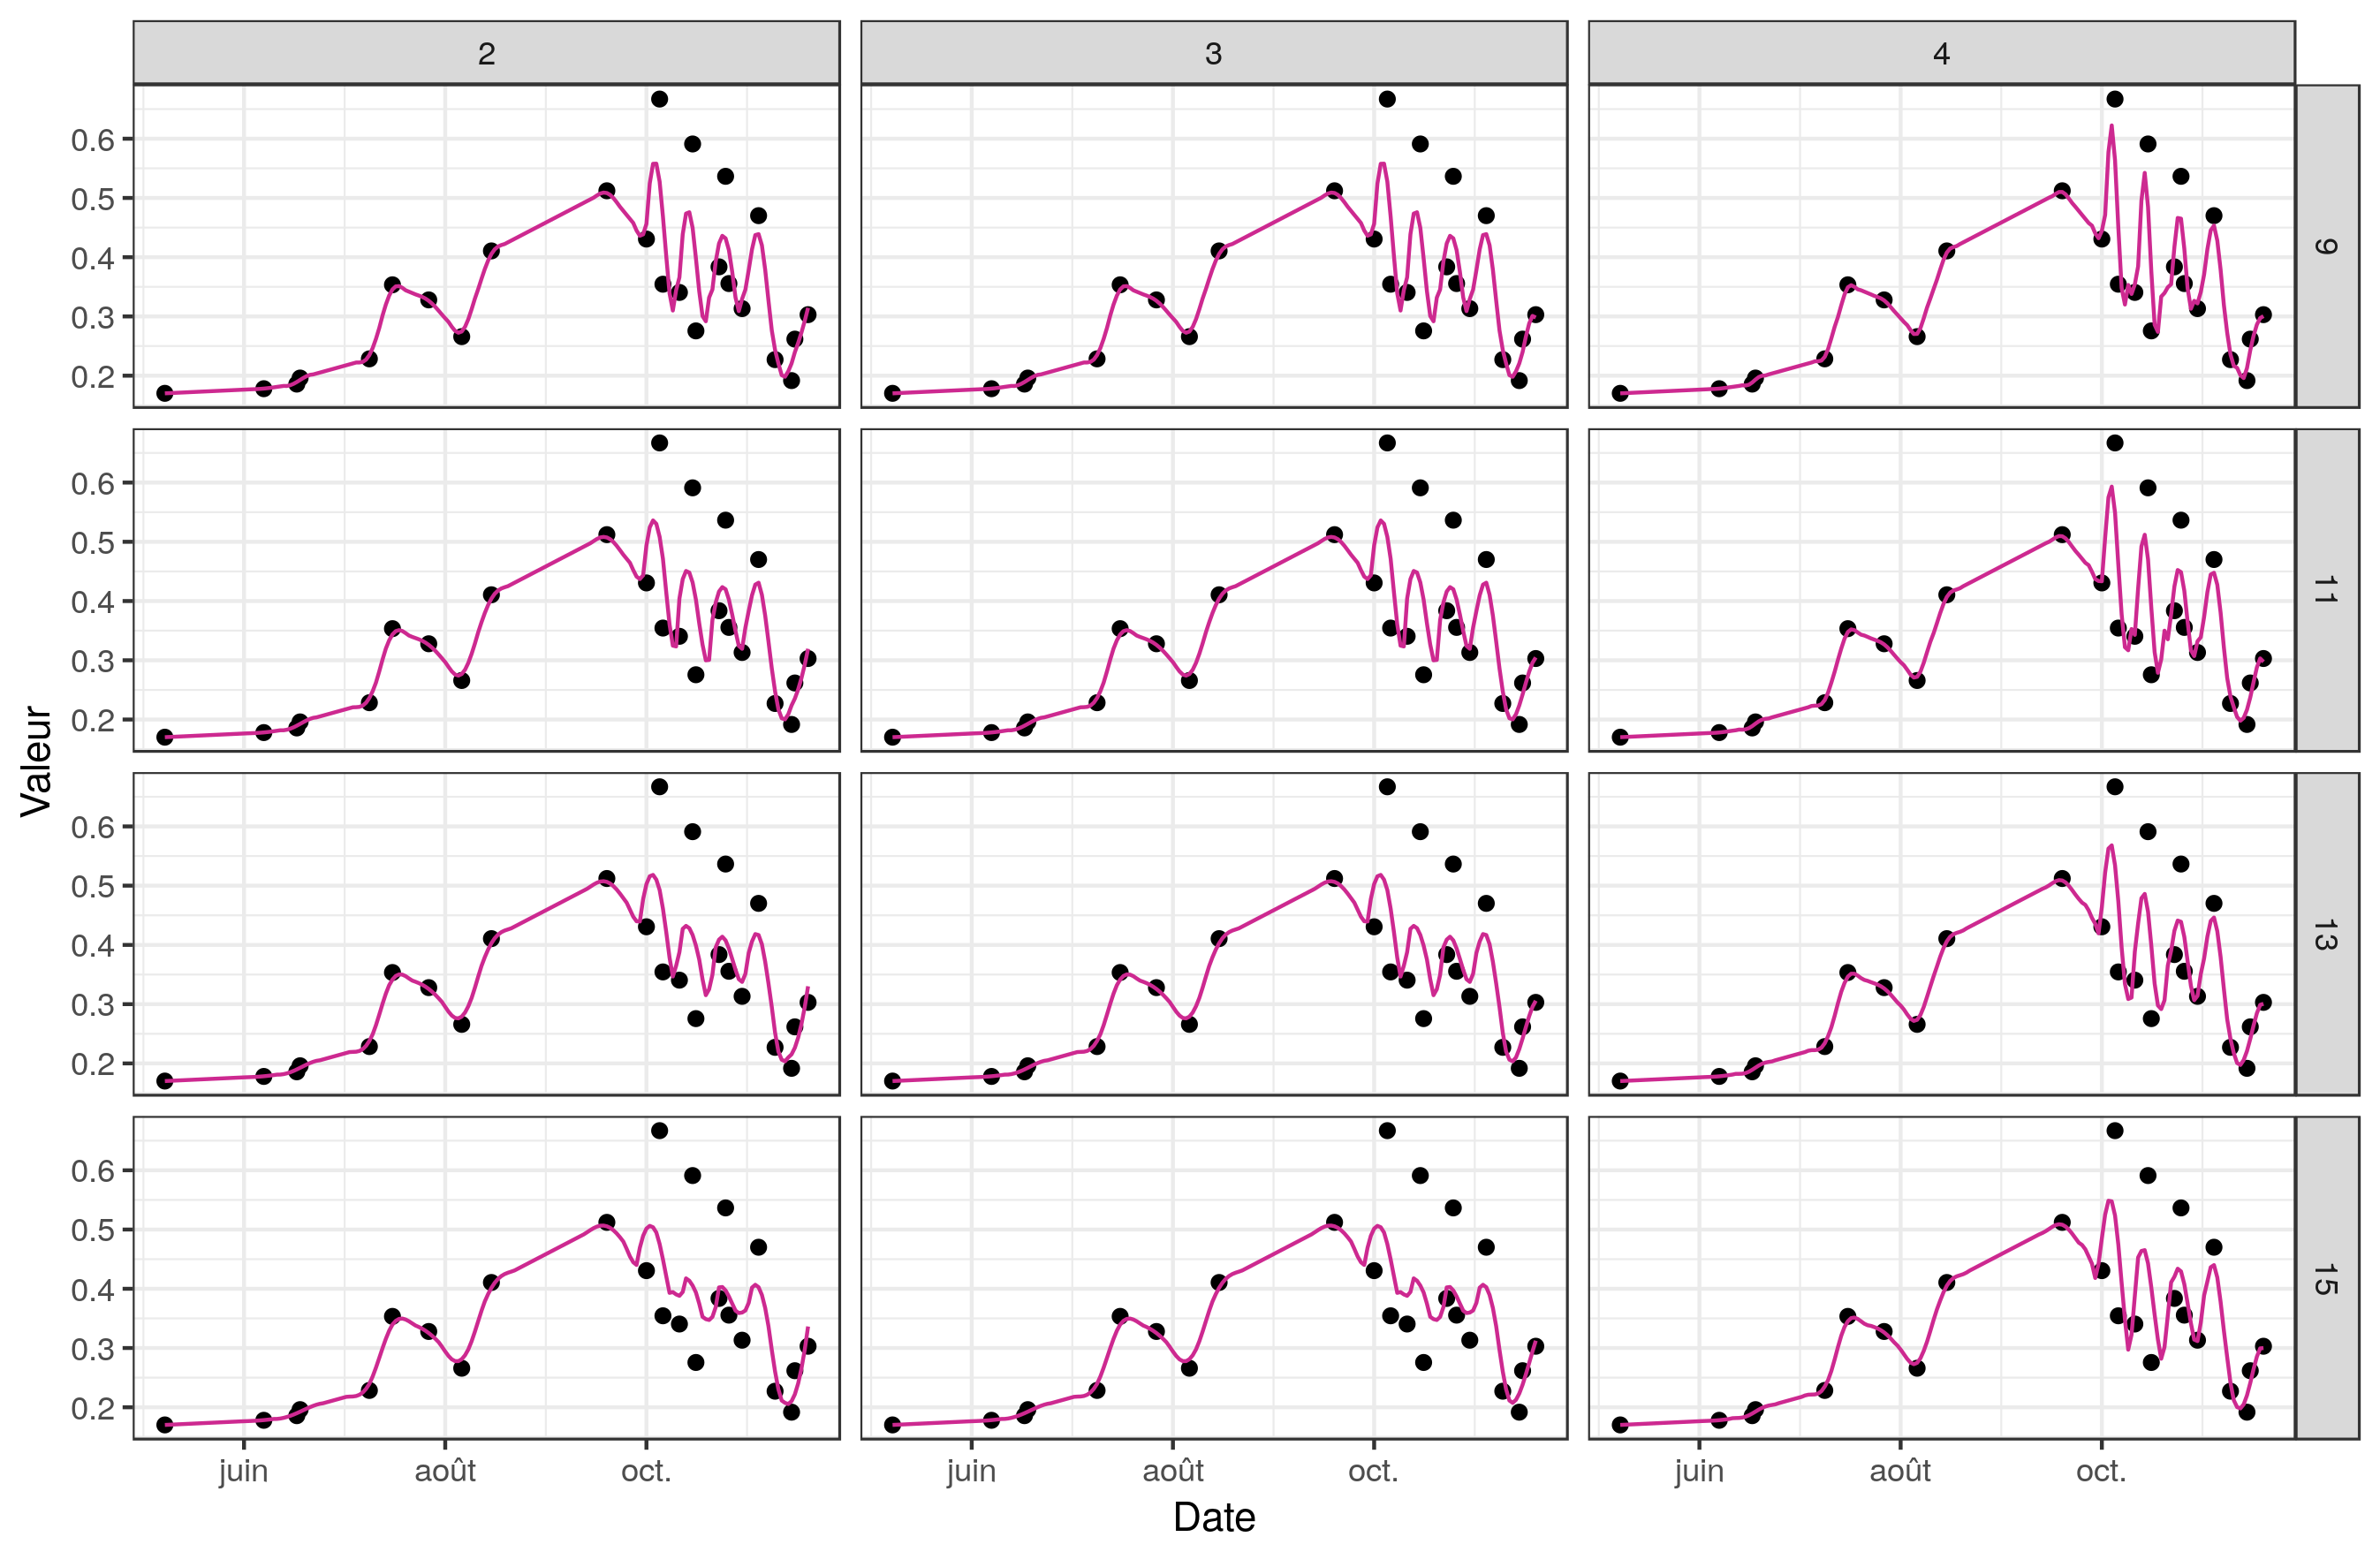
\includegraphics[scale=0.7]{annexes/savgol_prs_1.png} 
 \end{center}
 %\caption{Quelques résultats du lissage de la série temporelle rectifiée}
 %\label{fig-lissage-prscor}
\end{figure}

\begin{figure}[htbp]
 \begin{center}
  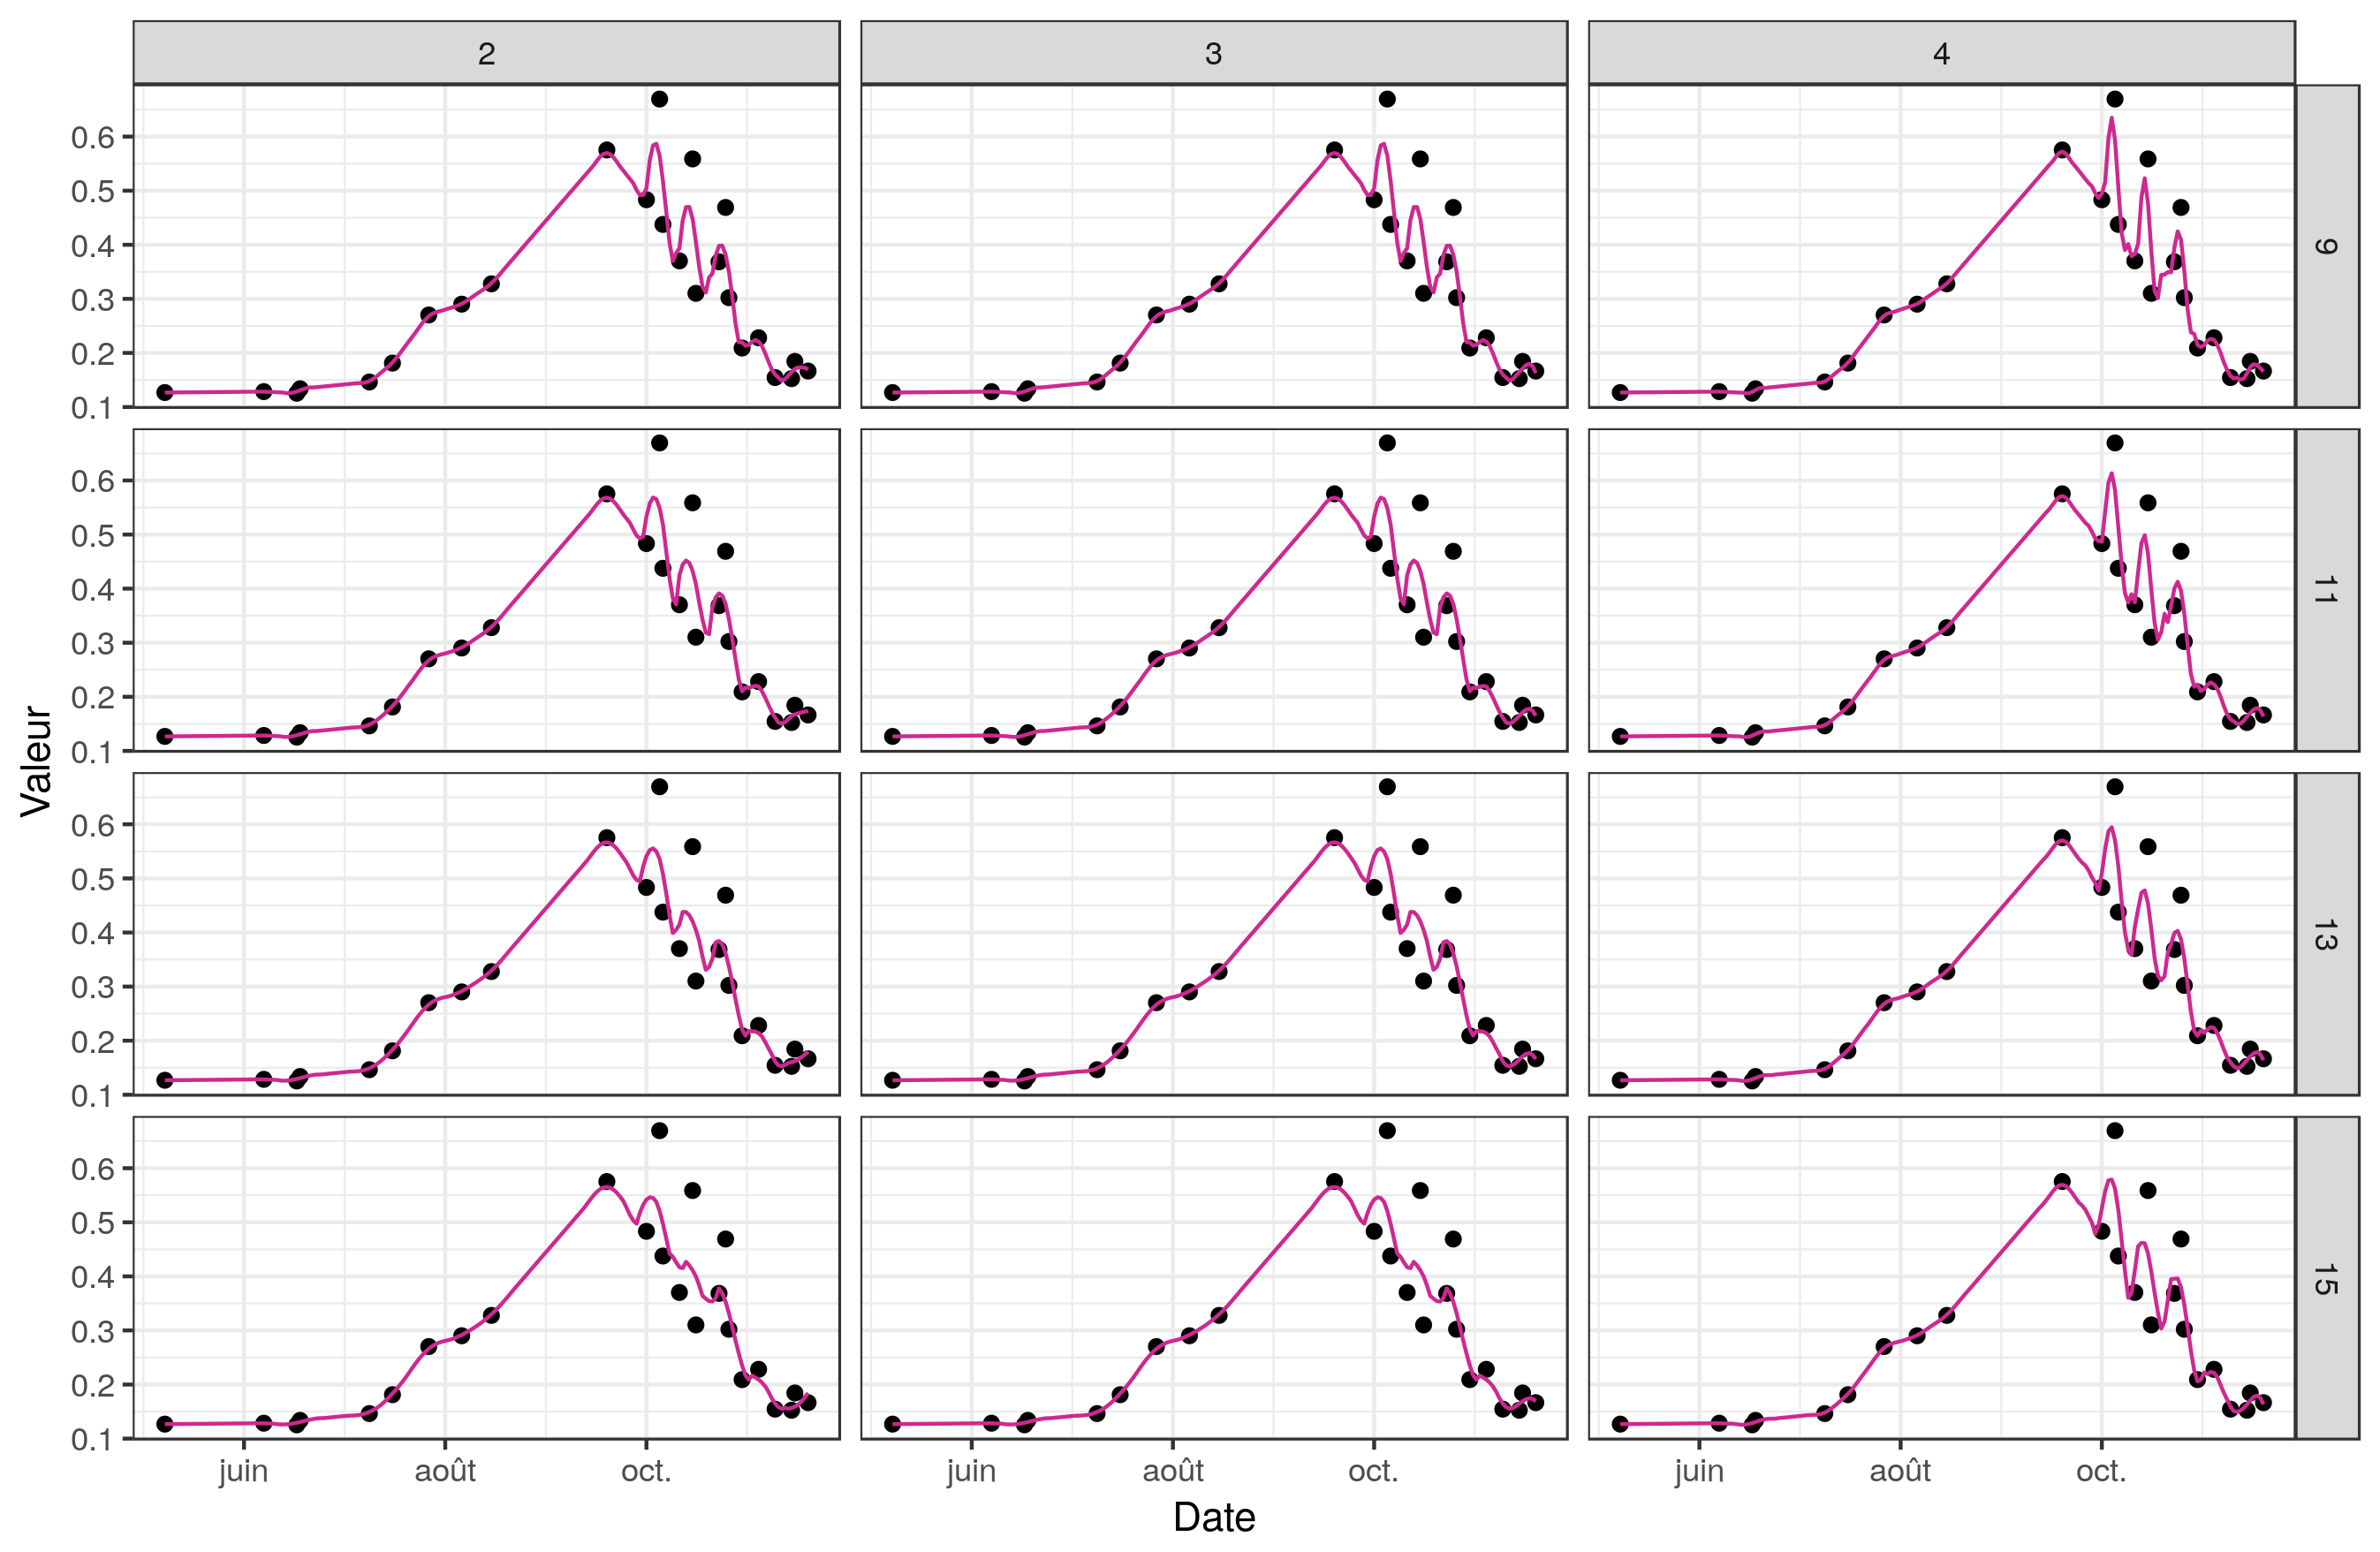
\includegraphics[scale=0.7]{annexes/savgol_prs_2.png} 
 \end{center}
 %\caption{Quelques résultats du lissage de la série temporelle rectifiée}
 %\label{fig-lissage-prscor}
\end{figure}

\begin{figure}[htbp]
 \begin{center}
  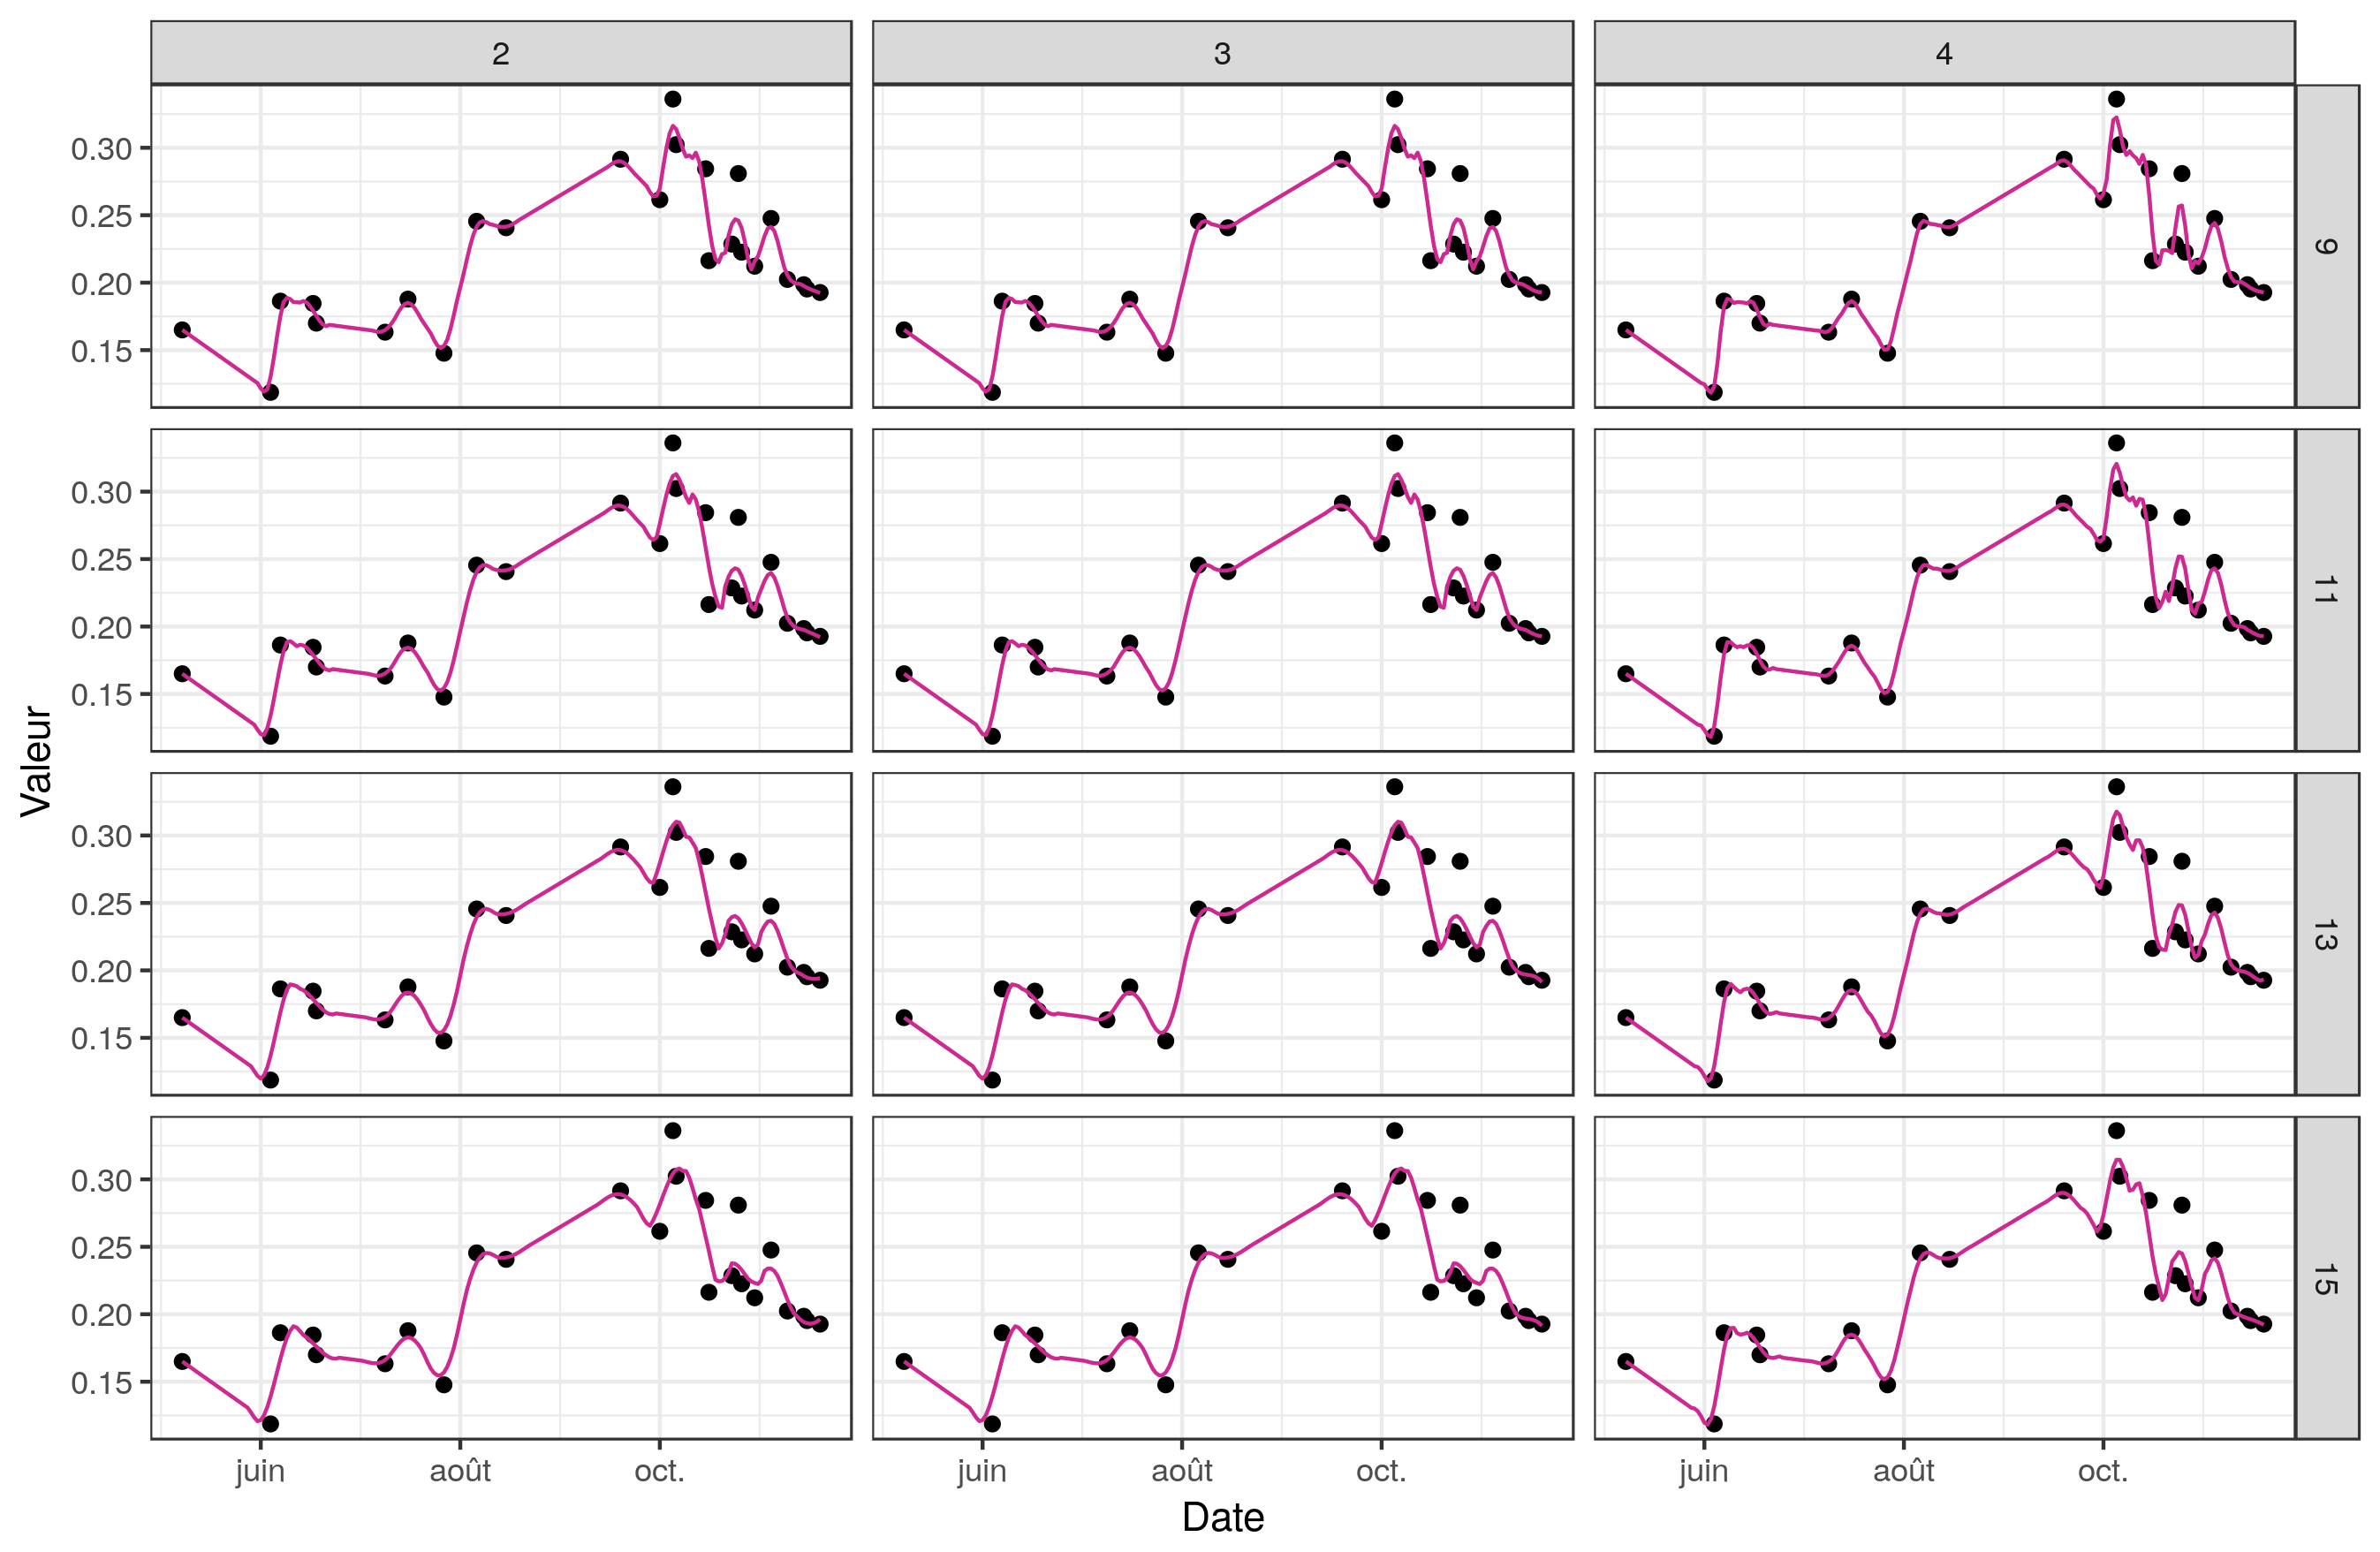
\includegraphics[scale=0.7]{annexes/savgol_prs_3.png} 
 \end{center}
 %\caption{Quelques résultats du lissage de la série temporelle rectifiée}
 %\label{fig-lissage-prscor}
\end{figure}

% \begin{figure}[htbp]
%  \begin{center}
%   \includegraphics[scale=0.7]{annexes/savgol_prscor_1.png} 
%  \end{center}
%  %\caption{Quelques résultats du lissage de la série temporelle rectifiée}
%  %\label{fig-lissage-prscor}
% \end{figure}
% 
% \begin{figure}[htbp]
%  \begin{center}
%   \includegraphics[scale=0.7]{annexes/savgol_prscor_2.png} 
%  \end{center}
%  %\caption{Quelques résultats du lissage de la série temporelle rectifiée}
%  %\label{fig-lissage-prscor}
% \end{figure}
% 
% \begin{figure}[htbp]
%  \begin{center}
%   \includegraphics[scale=0.7]{annexes/savgol_prscor_3.png} 
%  \end{center}
%  %\caption{Quelques résultats du lissage de la série temporelle rectifiée}
%  %\label{fig-lissage-prscor}
% \end{figure}
